%Be more precise about what the system should and should not satisfy.
%Be sure to use the vocabulary introduced in the problem analysis.
\chapter{Requirements specification}

\subsection{Gameplay}%Jonathan
We originally wanted to implement a rpg style platformer with:
\begin{enumerate}
\item Items
\item Hero leveling
\item Abilities
\item A decent story
\end{enumerate}
We quickly found out that the limited flash memory on the arduino would greatly limit what we could implement. We agreed on going back to the classics of arcade games. We decided to create a "rogue like" game and focus on increasing difficulty per level and having a high score as the intensive to play the game.

\subsubsection{High Score}
High scores is something you almost always see in arcade games or just smaller games. Its a great way to compare and compete and to show who's the best. 
To do this we were requierd to save data on the EEPROM which is the ´hard drive` of the arduino. This way the high score will never reset unless we want it to.

\subsubsection{Coins}
Coin were added as an additional game play element to broaden the game. The player now has an incentive to go explore the entirety of the map, since collecting coins is an easy way to get additional score.


\subsection{Timeplan} %Cebrail/Jonathan
When we started the `Fagprojekt' we used a time-plan that followed an non-agile development
system called waterfall. The waterfall system is a sequential design process.
It is designed to get through the project phases and have a product as soon as
possible. The phases in our project can be seen in the figure below.
The report is both written seamlessly and separately in the end of the project,
therefore it does not has to be illustrated, as it will create confusion.

\subsubsection{Waterfall}
When the waterfall ends and we still have time
we will go back to the start and check for new requirements
and the whole waterfall process starts again. You can check our waterfall
timeplan in the appendices, please
see Figure~\ref{fig:Waterfall_chart} for that.

\begin{figure}[h]
  \centering
  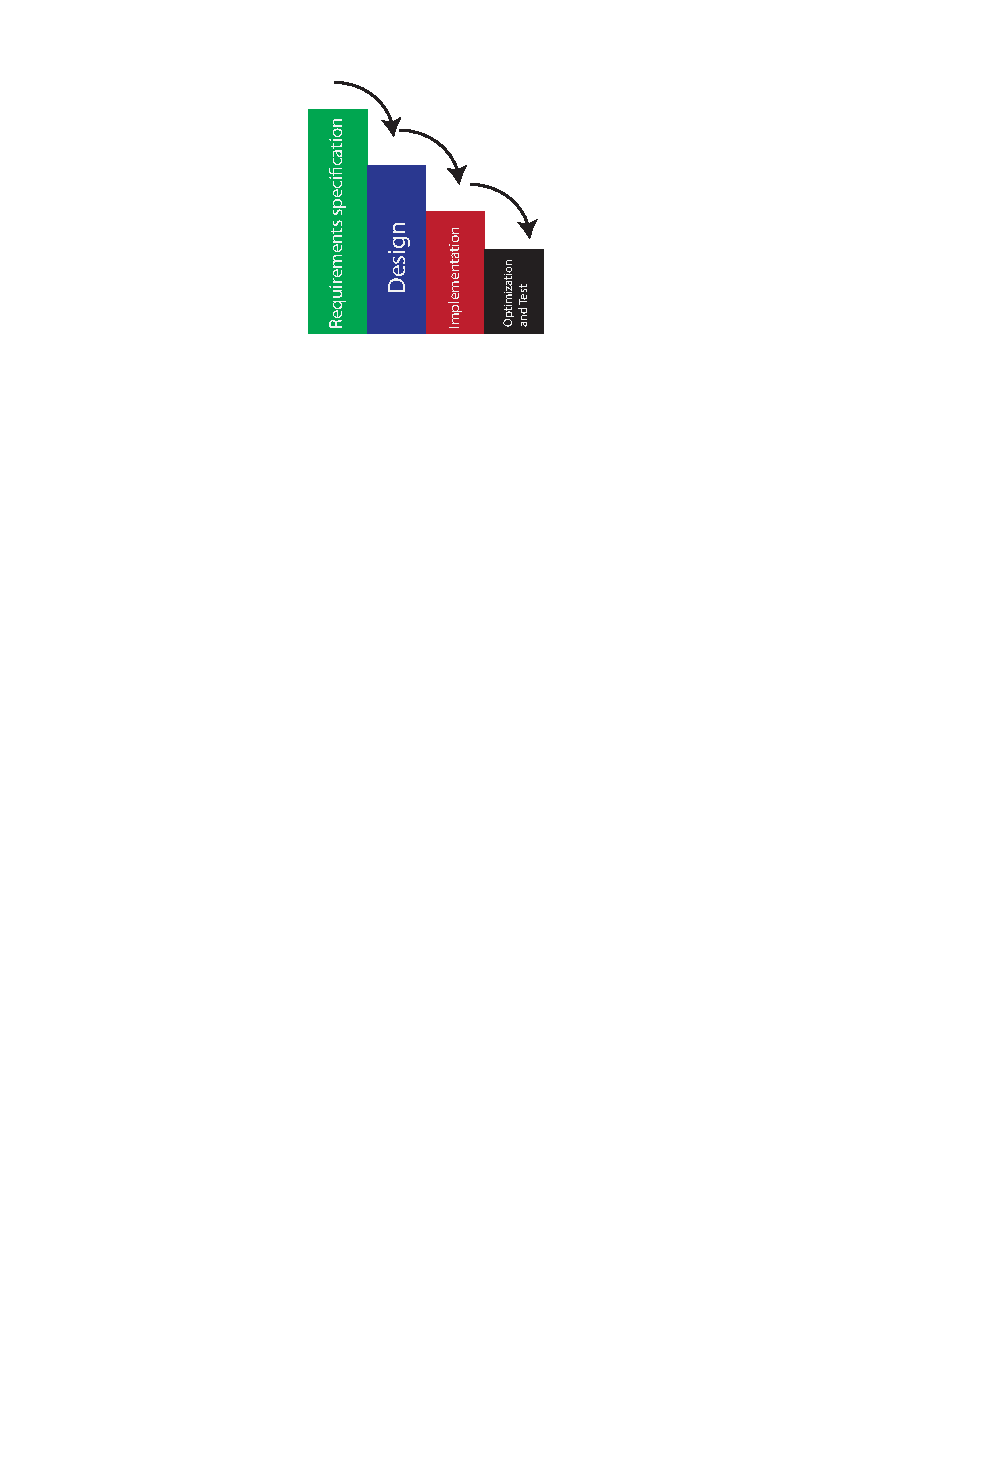
\includegraphics[scale=0.6]{Figures/Waterfall}
  \caption{An overview of the waterfall time plan.}
\label{fig:Waterfall}
\end{figure}
\subsection{Time Boxing} %Jonathan
We were conviced that using "Time Boxing" would be the way to go.
Timeboxing divides The schedule into a number of separate time periods(timeboxes), with each part having its own deliverables, deadline and budget.
Breaking bigger tasks into smaller tasks with better manageable time frames.
What also is important is that by the end of each timebox we need to have a product that if all else fails we can roll back and release our game from an earlier state. The following table shows the timeboxes we have created during the project.

% Please add the following required packages to your document preamble:
% \usepackage[table,xcdraw]{xcolor}
% If you use beamer only pass "xcolor=table" option, i.e. \documentclass[xcolor=table]{beamer}

\begin{table}[h]
\begin{tabular}{llll}
\rowcolor[HTML]{BBDAFF}
{\color[HTML]{000000} \textbf{week 8-10}} & {\color[HTML]{000000} \textbf{week 11-13}} & {\color[HTML]{000000} \textbf{week 14-15}} & {\color[HTML]{000000} \textbf{week 16-17}} \\
Code exercise                        & Enemies                               & Scene generation (simple)             & Graphics                              \\
Game design                          & Collision Detection                   & Player                                & Sprites                               \\
Class Design                         & AI                                    &                                       & Map generation                        \\
                                     & Input                                 &                                       &                                       \\
Report                               & Report                                & Report                                & Report                                \\
                                     &                                       &                                       &                                       \\
\rowcolor[HTML]{BBDAFF} 
\textbf{week 18-90}                       & \textbf{week 19}                           & \textbf{week 20}                           & \textbf{week 22-25}                        \\
Endgame                              & Scene generation                      & Sprites                               & Optimization                          \\
Map generation                       & Optimization                          & Sound                                 &                                       \\
                                     & Attack                                & Optimization                          &                                       \\
                                     &                                       & Animation                             &                                       \\
Report                               & Report                                & Report                                &                                      
\end{tabular}
\caption{The timeboxes are seperated per week}
\end{table}
